\documentclass[10pt]{beamer}
\usetheme{jambro}

\title[]{Macroeconomia I - Determinação de preços e taxa natural de desemprego}
\author[]{\href{https://pvfonseca.github.io}{Paulo Victor da Fonseca}}
\date{}

\hypersetup{
    colorlinks = true,
    urlcolor = teal,
    linkcolor = teal    
}
\usepackage[portuguese]{babel}
\usepackage{subfig}
\usepackage{emoji}
\usepackage{hyperref}

\begin{document}

\begin{frame}[plain]
    \titlepage{
        \begin{center}
            \begin{minipage}{0.8\textwidth}
                \centering
            \end{minipage}
        \end{center}}
\end{frame}

\begin{frame}{Sumário}
    \tableofcontents
\end{frame}

\section{Determinação de preços}
\begin{frame}
    {Determinação de preços}
    \begin{itemize}
        \item Preços fixados pelas firmas dependem, essecialmente, dos custos de produção incorridos\bigskip
        \item Os custos de produção, por sua vez, dependem de dois fatores:\medskip
        \begin{enumerate}
            \item Da natureza da função de produção, que formaliza a relação entre insumos utilizados na produção e a quantidade máxima de produto obtida\medskip
            \item Dos preços destes insumos, determinados no mercado de fatores
        \end{enumerate}
    \end{itemize}
\end{frame}

\begin{frame}
    {Determinação de preços}
    \begin{itemize}
        \item Por ora, vamos supor que firmas produzem bens usando trabalho como único fator de produção. Formalmente:
        \begin{equation}
            Y = AN,
        \end{equation}
        onde $Y$ é o produto, $N$ o nível de emprego e $A$ a produtividade do trabalho\bigskip
        \item A função de produção adotada implica que a produtividade do trabalho é constante e igual a $A$\bigskip
        \item Em termos microeconômicos, temos um caso de retornos constantes de escala ao trabalho na produção
    \end{itemize}
\end{frame}

\begin{frame}
    {Determinação de preços}
    \begin{itemize}
        \item Dada a hipótese de retornos constantes de escala, podemos normalizar o modelo e escolher unidades de produto de modo que um trabalhador produza uma unidade de produto\bigskip
        \item Formalmente:
        \begin{equation}
            Y = N
        \end{equation}
        \item Com isso, o custo de produzir uma unidade adicional de produto é igual ao custo de empregar um trabalhador adicional ao nível de salário nominal $W$\bigskip
        \item Ou seja, o custo marginal do produto é igual a $W$
    \end{itemize}
\end{frame}

\begin{frame}
    {Determinação de preços}
    \begin{itemize}
        \item Em um mercado de bens perfeitamente competitivo, teríamos o resultado clássico de que o preço de uma unidade de produto seria igual ao custo marginal de produção: $P = W$\bigskip
        \item No entanto, muitos mercados de bens não são perfeitamente competitivos e, nestes casos, as firmas fixam um preço acima do seu custo marginal\bigskip
        \item Uma maneira simples de modelar esse fato é supor que firmas fixam seu preço de acordo com a seguinte equação:
        \begin{equation}
            P = (1 + m)W,
        \end{equation}
        em que $m$ é a \hlight{margem (\emph{markup})} do preços sobre o custo
    \end{itemize}
\end{frame}

\section{Taxa natural de desemprego}
\begin{frame}
    {Introdução}
    \begin{itemize}
        \item Análise das implicações da determinação de salários e de preços sobre o desemprego\bigskip
        \item Para isso, adotaremos a hipótese de que salários nominais, $W$, dependem do nível de preços efetivo, $P$ (ao invés do nível de preços esperado, $P^e$). Formalmente:
        \begin{equation}
            P^e = P
        \end{equation}
        \item Sob essa hipótese, as relações de fixação de salários e de preços determinam a \hlight{taxa natural de desemprego} (ou taxa de desemprego de equilíbrio)
    \end{itemize}
\end{frame}

\begin{frame}
    {Relação de fixação de salários}
    \begin{itemize}
        \item Temos, portanto, a seguinte relação de fixação de salários:
        \begin{equation}
            W = PF(u,z)
        \end{equation}
        \item Como o salário relevante tanto para firmas quanto para trabalhadores é o salário real, é conveniente rearranjarmos a equação anterior:
        \begin{equation}
            \frac{W}{P} = F(u,z)
        \end{equation}
    \end{itemize}
\end{frame}

\begin{frame}
    {Relação de fixação de salários}
    \begin{itemize}
        \item A determinação de salários implica uma relação negativa entre salário real, $W/P$, e a taxa de desemprego, $u$\bigskip
        \item Intuição: quanto maior a taxa de desemprego, menor o poder de negociação dos trabalhadores e, portanto, menor o salário real
    \end{itemize}
\end{frame}

\begin{frame}
    {Relação de fixação de preços}
    \begin{itemize}
        \item Relação de fixação de preços:
        \begin{equation}
            P = (1 + m)W
        \end{equation}
        \item Portanto:
        \begin{equation}
            \frac{P}{W} = 1 + m,
        \end{equation}
        a razão entre nível de preços e salário nominal (razão produto-custo marginal) é igual a 1 mais o \emph{markup}\bigskip
        \item Em termos de salário real:
        \begin{equation}
            \frac{W}{P} = \frac{1}{1 + m}
        \end{equation}
    \end{itemize}
\end{frame}

\begin{frame}
    {Relação de fixação de preços}
    \begin{itemize}
        \item As decisões de fixação de preços determinam o salário real pago pelas empresas\bigskip
        \item Um aumento no \emph{markup} faz com que as empresas aumentem seus preços, a um dado nível de salário nominal que pagam aos trabalhadores\bigskip
        \item De modo equivalente, um aumento no \emph{markup} causa uma diminuição do salário real
    \end{itemize}
\end{frame}

\begin{frame}
    {Relação de fixação de preços}
    \begin{itemize}
        \item A relação inversa entre salário real e \emph{markup} pode não ser imediatamente intuitiva\bigskip
        \item Suponha que uma empresa individual aumente sua margem elevando, assim, o preço de seu produto\bigskip
        \item Neste caso, o salário real de seus funcionários não muda muito\bigskip
        \item Funcionários continuam recebendo o mesmo salário nominal, e o produto fabricado pela empresa é, no máximo, uma pequena parte de suas cestas de consumo
    \end{itemize}
\end{frame}

\begin{frame}
    {Relação de fixação de preços}
    \begin{itemize}
        \item Por outro lado, se o aumento de margem é generalizado, então, o aumento do nível de preços também será generalizado\bigskip
        \item Consequentemente, o salário real dos trabalhadores diminuirá - mesmo que os salários nominais permaneçam inalterados\bigskip
        \item Portanto, quanto maior a margem fixada pelas empresas, menor o salário real dos trabalhadores\bigskip
        \item O salário real resultante da fixação de preços é igual a $1/(1 + m)$ e, portanto, independe da taxa de desemprego 
    \end{itemize}
\end{frame}

\begin{frame}
    {Salários reais e taxa natural de desemprego}
    \begin{itemize}
        \item O equilíbrio no mercado de trabalho requer que o salário real determinado na fixação de salários seja igual ao salário real resultante da fixação de preços\bigskip
        \item Portanto, a \hlight{taxa natural de desemprego}, $u_n$, é aquela que satisfaz a condição de equilíbrio no mercado de trabalho:
        \begin{equation}
            F(u_n, z) = \frac{1}{1 + m}
        \end{equation}        
    \end{itemize}
\end{frame}

\begin{frame}
    {Salários reais e taxa natural de desemprego}
    \begin{center}
		\begin{minipage}[b]{.6\textwidth}
			\begin{tikzpicture}
				\node[inner sep=0, align=left] (image) at (0,0) {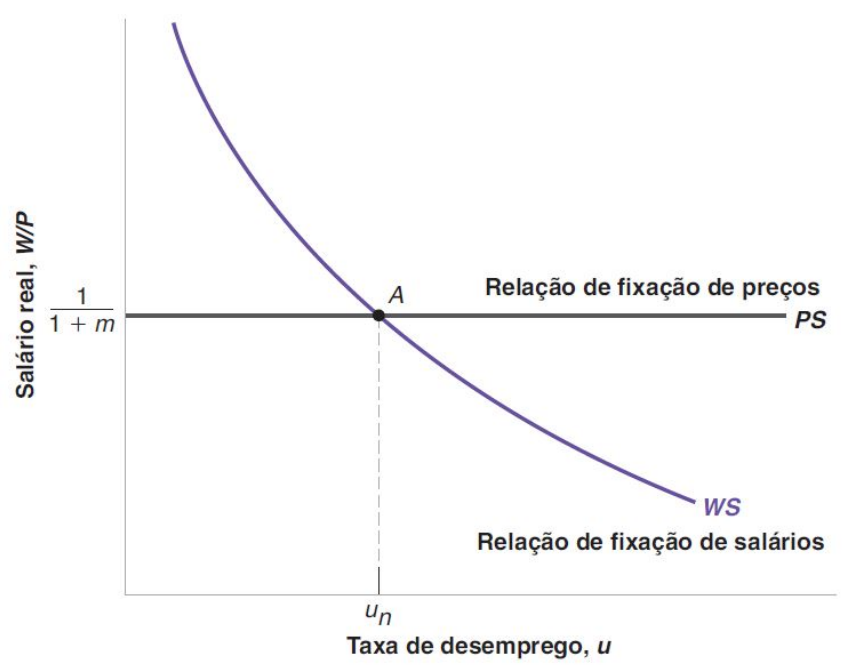
\includegraphics[width=\textwidth]{./figures/aula11_fig1.PNG}};
			\end{tikzpicture}
			\tiny{{\scshape FIGURA}. \ Salários, preços e taxa natural de desemprego. Fonte: Blanchard (2017)} 
		\end{minipage}
	\end{center}
\end{frame}

\begin{frame}
    {Salários reais e taxa natural de desemprego}
    \begin{itemize}
        \item As posições das curvas de fixação de salários e de fixação de preços (e, consequentemente, a taxa de desemprego de equilíbrio) dependem tanto de $z$ quanto de $m$\bigskip
        \item Portanto, a taxa "natural" de desemprego é afetada por instituições e políticas econômicas
    \end{itemize}
\end{frame}

\begin{frame}
    {Salários reais e taxa natural de desemprego}
    \begin{center}
		\begin{minipage}[b]{.5\textwidth}
			\begin{tikzpicture}
				\node[inner sep=0, align=left] (image) at (0,0) {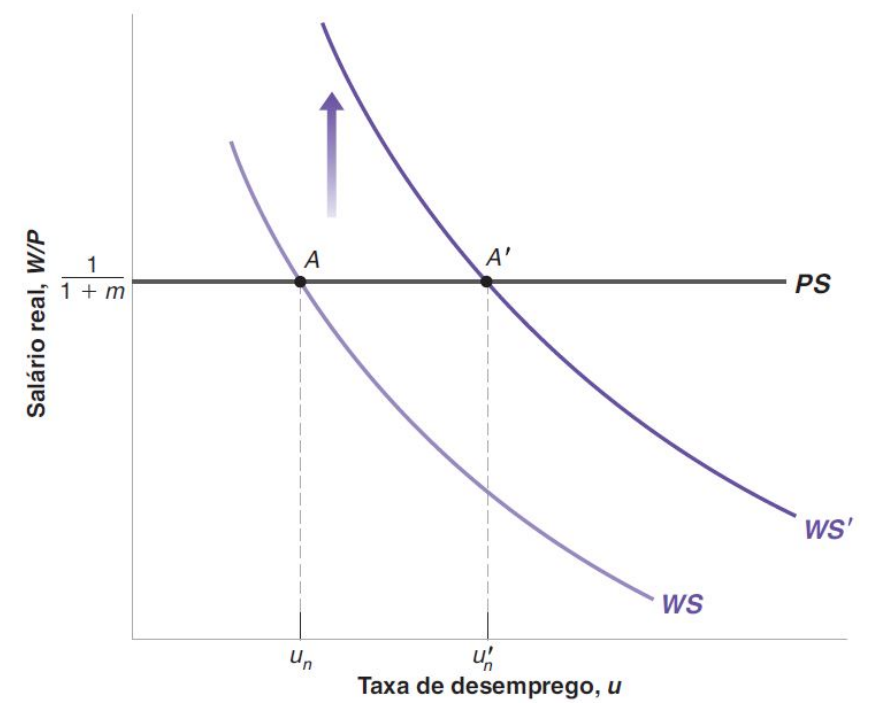
\includegraphics[width=\textwidth]{./figures/aula11_fig2.PNG}};
			\end{tikzpicture}
			\tiny{{\scshape FIGURA}. \ Seguro-desemprego e taxa natural de desemprego. Fonte: Blanchard (2017)} 
		\end{minipage}
	\end{center}
\end{frame}

\begin{frame}
    {Salários reais e taxa natural de desemprego}
    \begin{itemize}
        \item Aumento do seguro-desemprego torna perspectiva de desemprego mesos dolorosa e, portanto, aumenta salário determinado por fixadores de salários a uma dada taxa de desemprego\bigskip
        \item Portanto, a relação de fixação de salários WS (\emph{wage setting}) desloca-se para cima\bigskip
        \item Economia se move sobre a linha de fixação de preços PS (\emph{price setting}) - $A \to A'$\bigskip
        \item No novo ponto de equilíbrio, a taxa natural de desemprego aumenta $u_n \to \uparrow u_n'$\bigskip
        \item Em resumo, a uma dada taxa de desemprego, um seguro-desemprego maior leva a um salário real maior\bigskip
        \item Portanto, uma taxa de desemprego maior é necessária para trazer o salário real de volta ao que as firmas estão dispostas a pagar\bigskip
        \item I.e., um desemprego maior é um \hlight{dispositivo de disciplina} que obriga os salários a corresponderem ao que as firmas estão dispostas a pagar
    \end{itemize}
\end{frame}

\begin{frame}
    {Salários reais e taxa natural de desemprego}
    \begin{center}
		\begin{minipage}[b]{.5\textwidth}
			\begin{tikzpicture}
				\node[inner sep=0, align=left] (image) at (0,0) {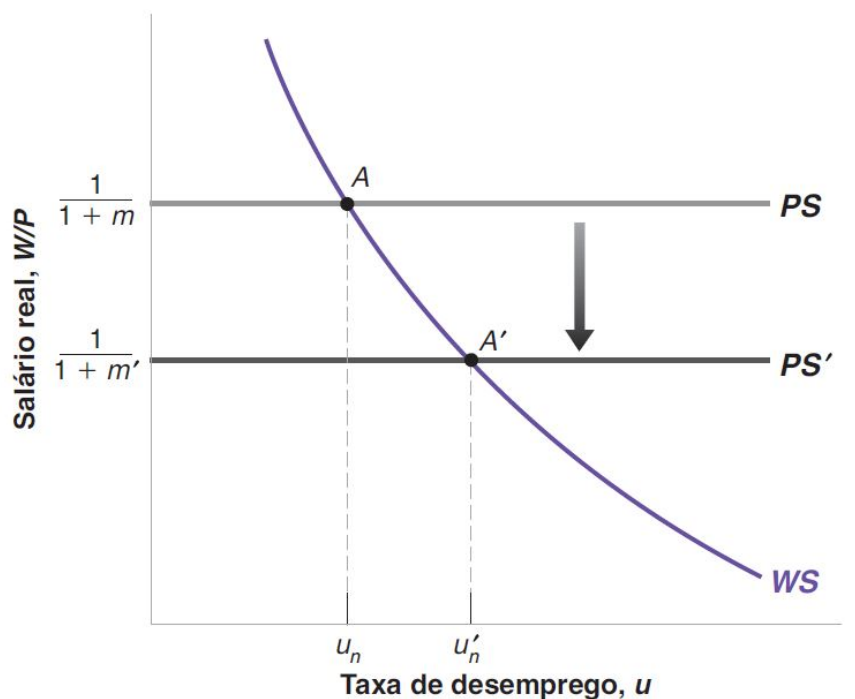
\includegraphics[width=\textwidth]{./figures/aula11_fig3.PNG}};
			\end{tikzpicture}
			\tiny{{\scshape FIGURA}. \ \emph{Markup} e taxa natural de desemprego. Fonte: Blanchard (2017)} 
		\end{minipage}
	\end{center}
\end{frame}

\begin{frame}
    {Salários reais e taxa natural de desemprego}
    \begin{itemize}
        \item \textcolor{purple}{Cumprimento menos rigoroso da legislação antitruste}. Menor rigor permite que empresas formem cartéis mais facilmente e aumentem seu poder de mercado - elevando o \emph{markup}, $m$\bigskip
        \item O aumento do \emph{markup} implica em uma redução do salário real pago pelas firmas, deslocando relação de fixação de preços para baixo $PS \to PS'$\bigskip
        \item Economia se move sobre WS e o equilíbrio de $A \to A'$\bigskip
        \item No novo ponto de equilíbrio, a taxa natural de desemprego aumenta de $u_n$ para $u_n'$\bigskip
        \item Ao permitir uma elevação de preços, dado o salário, o cumprimento menos rigoroso da legislação antitruste leva a uma diminuição do salário real\bigskip
        \item Portanto, um nível de desemprego maior é necessário para fazer funcionários aceitarem esse salário menos, levando a um aumento da taxa natural de desemprego
    \end{itemize}
\end{frame}

\section{Considerações finais}
\begin{frame}
    {Considerações finais}
    \begin{itemize}
        \item Vimos que o equilíbrio no mercado de trabalho determina a taxa de desemprego de equilíbrio e, consequentemente, o nível de produto (via função de produção)\bigskip
        \item Pergunta óbvia: por que dedicamos tanto tempo ao estudo da demanda agregada e mercado de bens e serviços?\bigskip
        \item E quanto às conclusões anteriores de que o nível de produto agregado era determinado por fatores como políticas fiscal e monetária, confiança do consumidor, etc.?\bigskip
        \item A resposta a essas perguntas está na diferença entre \hlight{curto prazo} e \hlight{médio prazo}
    \end{itemize}
\end{frame}

\begin{frame}
    {Considerações finais}
    \begin{itemize}
        \item Taxa natural de desemprego e níveis associados de emprego e produto agregados derivados sob duas hipóteses:\medskip
        \begin{enumerate}
            \item Equilíbrio no mercado de trabalho\medskip
            \item Igualdade entre nível de preços efetivo e esperado\bigskip
        \end{enumerate}
        \item No entanto, não há razões para que a segunda hipótese seja verdadeira no curto prazo\bigskip
        \item O nível de preços pode ser diferente do que era esperado quando os salários nominais foram fixados\bigskip
        \NB{Portanto, no curto prazo n\~{a}o h\'{a} motivo para que o desemprego seja igual \`{a} taxa natural, ou para que o produto seja igual a seu n\'{i}vel natural}
    \end{itemize}
\end{frame}

\begin{frame}
    {Considerações finais}
    \begin{itemize}
        \item No entanto, é pouco provável que as expectativas dos agentes estejam sistematicamente erradas (e.g., sempre muito altas ou muito baixas)\bigskip
        \item É por isso que, no médio prazo, o desemprego tende a retornar à taxa natural, e o produto tende a retornar ao seu nível natural\bigskip
        \item Temos, então, conforme veremos de forma mais detalhada a seguir, que no curto prazo os fatores que determinam os movimentos do produto são, de fato, os que estudamos anteriormente\bigskip
        \item Já para o médio prazo, os fatores que determinam o desemprego e o produto agregados são os que acabamos de ver (poder de mercado, seguro-desemprego, etc.)
    \end{itemize}
\end{frame}

\section{Bibliografia}
\begin{frame}{\emoji{books} Bibliografia}
    \begin{itemize}                
        \item BLANCHARD, O. Macroeconomia. 7.ed. São Paulo: Pearson Education do Brasil, 2017\medskip                
        \item CARLIN, W.; SOSKICE, D. Macroeconomics: Institutions, instability, and the financial system. Oxford, UK: Oxford University Press, 2015\medskip        
    \end{itemize}
\end{frame}
\end{document}